\section{Anwendungen in der anorganischen Chemie}
\subsection{[SIMesPGa\textit{t}Bu$_2$]$_2$, [SIMesP(Ga\textit{t}Bu$_2$)$_2$Cl] und [K(SIMesP)$_3$Al\textit{t}Bu]}
\subsection{[Hg$_8$Te$_8$(Te$_2$)$_4$]$^{8-}$: Ein anorganisches Porphyrin?}
\begin{figure}[ht!]
	\centering
	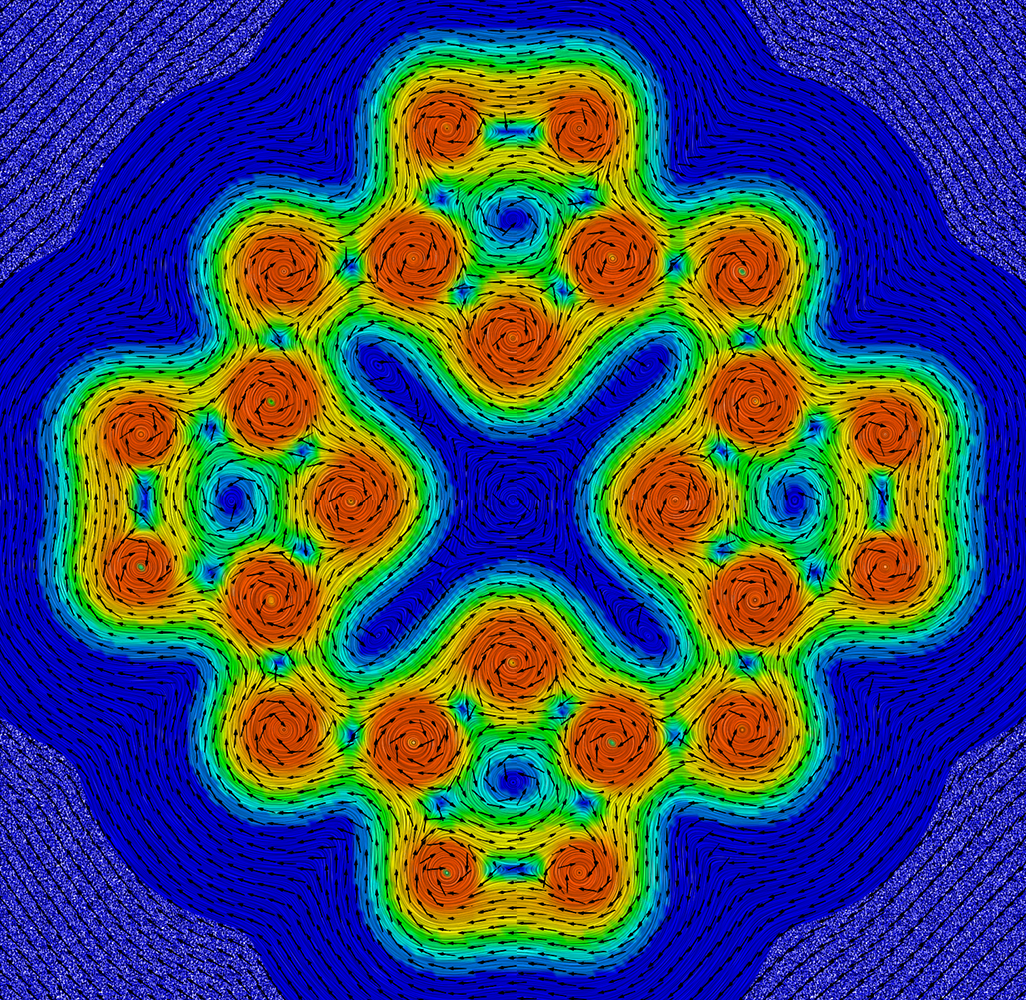
\includegraphics[width=0.6\textwidth]{hgte_1bohr}
	\captionsetup{figurewithin = chapter}
	\captionsetup{font=small, labelfont=bf}\caption{Ringströme von $[$Hg$_8$Te$_8$(Te$_2$)$_4]^{8-}$}{Ringströme von $[$Hg$_8$Te$_8$(Te$_2$)$_4]^{8-}$ \unit[1]{bohr} oberhalb der Molekülebene, dargestellt zwischen \unit[0]{a.u.} (blau) und \unit[0.07]{a.u.}.}
\label{abb:hgtelic}
\end{figure}

\begin{figure}[ht!]
	\centering
	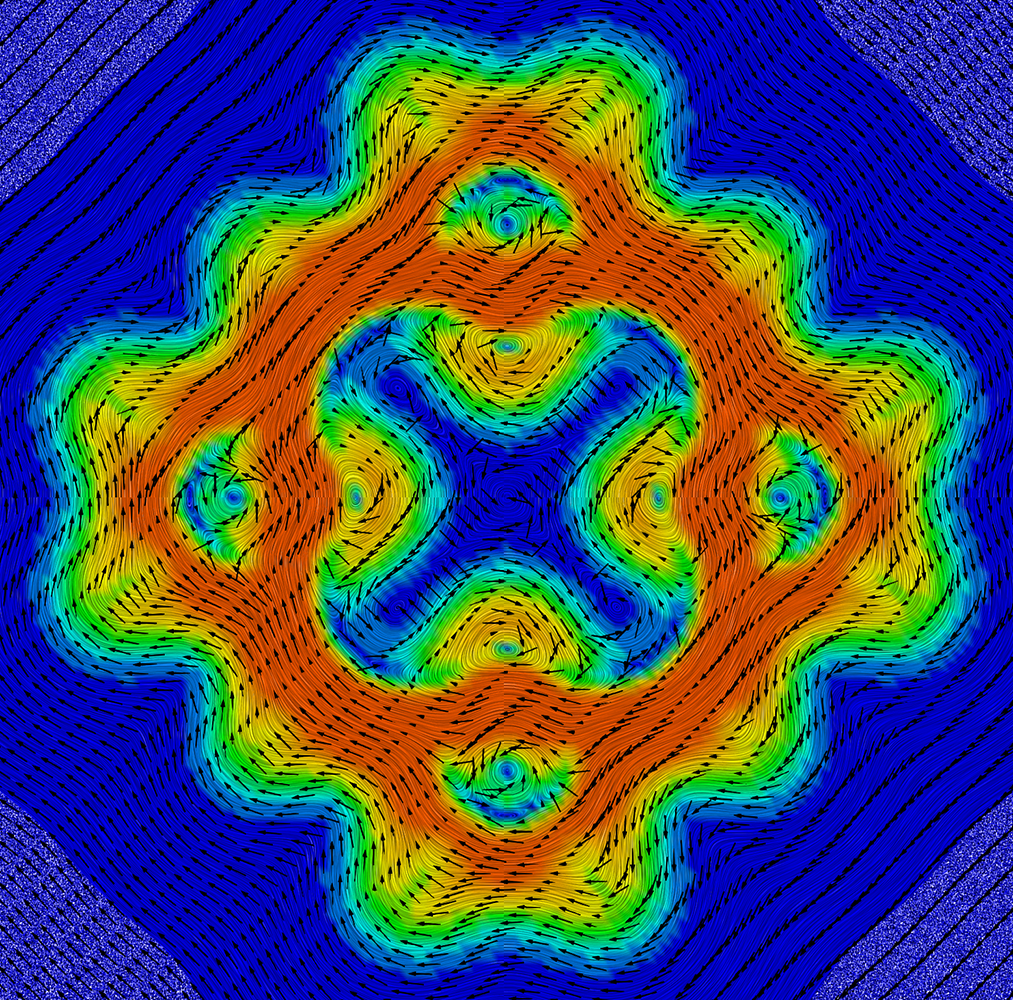
\includegraphics[width=0.6\textwidth]{porph_1bohr}
	\captionsetup{figurewithin = chapter}
	\captionsetup{font=small, labelfont=bf}\caption[Ringströme von Porphyrin]{Ringströme von Porphyrin \unit[1]{bohr} oberhalb der Molekülebene, dargestellt zwischen \unit[0]{a.u.} (blau) und \unit[0.07]{a.u.}.}
\label{abb:porphlic}
\end{figure}

\begin{figure}[ht!]
	\centering
	\includegraphics[width=0.6\textwidth]{b8s16_1bohr}
	\captionsetup{figurewithin = chapter}
	\captionsetup{font=small, labelfont=bf}\caption[Ringströme von B$_8$S$_{16}$]{Ringströme von B$_8$S$_{16}$ \unit[1]{bohr} oberhalb der Molekülebene, dargestellt zwischen \unit[0]{a.u.} (blau) und \unit[0.07]{a.u.}.}
\label{abb:b8s16hlic}
\end{figure}

\begin{figure}[ht!]
	\centering
	\includegraphics[width=0.6\textwidth]{b8se16_1bohr}
	\captionsetup{figurewithin = chapter}
	\captionsetup{font=small, labelfont=bf}\caption[Ringströme von B$_8$Se$_{16}$]{Ringströme von B$_8$Se$_{16}$ \unit[1]{bohr} oberhalb der Molekülebene, dargestellt zwischen \unit[0]{a.u.} (blau) und \unit[0.07]{a.u.}.}
\label{abb:b8se16hlic}
\end{figure}
\subsection{[Co\@Sn$_6$Sb$_6$]$^{3-}$}
\section{Ringströme in großen ringförmigen Kohlenstoffnanoröhren}